\documentclass[11pt]{article}
\usepackage[a4paper,margin=1in]{geometry}
\usepackage{amsmath,amssymb}
\usepackage{graphicx}
\usepackage{booktabs}
\usepackage{caption}
\usepackage{subcaption}
\usepackage{float}
\usepackage{xcolor}
\usepackage[hidelinks]{hyperref}
\usepackage{enumitem}
\usepackage{parskip}
\title{\textbf{Digital Image Processing --- Assignment 2}\\[0.3em]\large Problem 4: Edge-Preserving Smoothing: Bilateral vs. Kuwahara}
\author{Ujjwal Gupta}
\date{\today}
\begin{document}
\maketitle
\tableofcontents
\vspace{1em}

\section{Introduction / Problem Statement}

Problem 4 of the assignment (worth 15 of the 100 total marks) asks for an in-depth
comparison of two classical \emph{edge-preserving} spatial smoothing filters -- the
bilateral filter and the Kuwahara filter -- across three sub-parts:

\begin{itemize}[leftmargin=1.5em]
  \item \textbf{4.1 Implementation and matched-strength comparison (7 pts).}
  Implement both filters from scratch, formulate and justify a mathematical
  definition of ``matched effective smoothing strength'' between them, and evaluate
  both against a clean ground-truth image using PSNR and SSIM, with cropped
  zoomed-in boundary comparisons.
  \item \textbf{4.2 Mitigating Kuwahara blockiness and complexity analysis (5 pts).}
  Explain why classical Kuwahara's hard $\arg\min$ selection specifically produces
  blocky, ``painterly'' artefacts (rather than blur or ringing); implement one
  structural modification that mitigates this; and provide a per-pixel operation-count
  complexity analysis for all three filters (classical Kuwahara, the modification,
  and bilateral).
  \item \textbf{4.3 Quantitative breakdown analysis of bilateral filtering (3 pts).}
  Programmatically generate synthetic step-edge test images across a controlled
  gradient of Noise-to-Contrast Ratios (NCR $=\sigma_{\text{noise}}/|\Delta I|$),
  identify the critical threshold $\text{NCR}^*$ at which the bilateral filter
  transitions from edge preservation to cross-edge smoothing, and explain the
  breakdown mathematically in terms of the range kernel.
\end{itemize}

This problem matters because linear smoothing (e.g.\ a Gaussian low-pass filter) is
fundamentally unable to reduce noise without also blurring genuine edges, since it
weights every neighbouring pixel by spatial proximity alone, with no regard for
whether that neighbour lies on the same side of a boundary. Bilateral and Kuwahara
filtering are two structurally different answers to the same problem -- one continuous
and range-weighted, one discrete and selection-based -- and understanding their
different failure modes (bilateral's gradual breakdown under high noise-to-contrast
ratio, Kuwahara's blocky artefacts from hard window selection) is central to
understanding edge-preserving filtering as a topic.

\section{Theoretical Background}

\subsection{The bilateral filter: joint spatial/range Gaussian weighting}

The bilateral filter computes, at each pixel $(x,y)$, a weighted average of
neighbouring pixels $(x',y')$ in which the weight is the product of two Gaussian
kernels: one in the \emph{spatial} domain (favouring nearby pixels), and one in the
\emph{range} (intensity) domain (favouring pixels of similar intensity):

\begin{align}
  \hat I(x,y) &= \frac{1}{W(x,y)}\sum_{(x',y')\in\Omega}
  I(x',y')\, w_s(x,y,x',y')\, w_r\big(I(x,y)-I(x',y')\big), \\
  w_s(x,y,x',y') &= \exp\!\left(-\frac{(x-x')^2+(y-y')^2}{2\sigma_s^2}\right), \\
  w_r(\Delta I) &= \exp\!\left(-\frac{\Delta I^2}{2\sigma_r^2}\right), \\
  W(x,y) &= \sum_{(x',y')\in\Omega} w_s(x,y,x',y')\, w_r\big(I(x,y)-I(x',y')\big),
  \label{eq:bilateral}
\end{align}

where $\Omega$ is a local window around $(x,y)$ and $W(x,y)$ is the per-pixel
normalisation that keeps $\hat I$ a proper weighted average. The spatial Gaussian
$w_s$ alone, applied without $w_r$, is exactly an ordinary Gaussian blur: it treats
every neighbour the same regardless of intensity and therefore blurs across edges.
The range Gaussian $w_r$ is what gives the filter its edge-preserving property: when
$(x',y')$ lies on the opposite side of a true edge from $(x,y)$, the intensity
difference $\Delta I = I(x,y)-I(x',y')$ is large relative to $\sigma_r$, so
$w_r(\Delta I)\approx 0$ and that neighbour is effectively excluded from the average
no matter how spatially close it is -- while same-side neighbours, whose intensity
differences are small (ideally dominated only by noise), retain near-full weight.
$\sigma_s$ controls the spatial extent of smoothing (analogous to a Gaussian blur's
kernel width) and $\sigma_r$ controls how aggressively intensity differences are
penalised -- a small $\sigma_r$ makes the filter very edge-sensitive but denoises
less; a large $\sigma_r$ denoises more but risks blending across real edges.

\subsection{The classical Kuwahara filter: sub-window variance selection}

The classical Kuwahara filter takes a different, non-Gaussian approach. At each pixel,
four overlapping square sub-windows $Q_1,Q_2,Q_3,Q_4$ (e.g.\ the four quadrants of a
larger window, each anchored at the centre pixel) are examined, and the filter outputs
the \emph{mean} of whichever sub-window has the \emph{minimal intensity variance}:
\begin{align}
  q^\star &= \operatorname*{arg\,min}_{q\in\{1,2,3,4\}} \operatorname{Var}(Q_q), \\
  \hat I(x,y) &= \operatorname{Mean}(Q_{q^\star}).
  \label{eq:kuwahara}
\end{align}
The intuition is that near a true edge, three of the four candidate sub-windows will
straddle the boundary (high variance, mixing both sides) while at least one sub-window
will lie entirely on one homogeneous side of the boundary (low variance); selecting
the minimum-variance sub-window therefore tends to average only within one side of an
edge, never across it, giving genuine edge preservation rather than a soft trade-off.

\subsubsection{Why hard $\arg\min$ selection causes blockiness, not blur or ringing}

Classical Kuwahara's output at a pixel is determined entirely by \emph{which} of the
four candidate sub-windows is selected by the hard $\arg\min$ in Eq.~\eqref{eq:kuwahara}.
As the pixel position slides across the image, the \emph{identity} of the
minimum-variance sub-window can flip discontinuously from one pixel to the next,
whenever two sub-windows' variances cross over -- and each flip switches the output to
a \emph{different} sub-window's mean, which is itself generally a different number.
The output is therefore a piecewise-constant mosaic of whichever sub-window ``won'' in
each local neighbourhood, with sharp jumps exactly at the boundaries between
``win regions'' -- a discontinuity introduced by the \emph{selection rule itself},
independent of whether the underlying image content actually has an edge there. This is
structurally different from:
\begin{itemize}[leftmargin=1.5em]
  \item \textbf{Blur}, which arises from \emph{continuous} averaging: the output changes
  smoothly as the window slides, with no discontinuity introduced by the operation
  itself;
  \item \textbf{Ringing}, which arises from a \emph{sharp frequency-domain cutoff}
  (as studied for ideal low-pass filters elsewhere in this assignment): oscillatory
  over/undershoot around a \emph{true} edge, not a new false edge appearing in a region
  that was originally flat.
\end{itemize}
Kuwahara's blockiness is thus a discontinuity artefact of the \emph{selection}
operation, producing new, spurious piecewise-constant boundaries (``tiles'') even
inside genuinely flat regions, wherever two sub-windows' noise-driven variances happen
to cross as the window slides across the image.

\subsection{Soft-Kuwahara: softmax reformulation}

The PDF-sanctioned de-blocking modification used here replaces the hard $\arg\min$
selection with a continuous \emph{softmax} weighting over all four sub-window means,
parameterised by a temperature $T$:
\begin{align}
  \omega_q &= \frac{\exp(-\operatorname{Var}(Q_q)/T)}{\sum_{q'=1}^{4}\exp(-\operatorname{Var}(Q_{q'})/T)},
  \qquad q=1,\dots,4, \\
  \hat I(x,y) &= \sum_{q=1}^{4} \omega_q \cdot \operatorname{Mean}(Q_q).
  \label{eq:softkuwahara}
\end{align}
As $T\to 0$, $\omega_{q^\star}\to 1$ for the minimum-variance sub-window and the
expression reduces exactly to the classical hard-selection rule; as $T\to\infty$, all
four weights tend to $1/4$ and the filter approaches a simple four-sub-window average.
At a finite, moderate $T$, as the pixel slides and the relative sub-window variances
change, the softmax weights shift \emph{continuously} rather than snapping discretely
between one-hot selections -- directly removing the mechanism identified above as the
source of blockiness, at the cost of smoothing the hard edge-selection behaviour
somewhat.

\subsection{Range-kernel breakdown analysis}

The bilateral filter's edge-preservation relies entirely on the range kernel
$w_r(\Delta I)=\exp(-\Delta I^2/2\sigma_r^2)$ being able to discriminate between the
typical intensity difference seen across a true edge and the typical intensity
difference seen between two noisy samples on the \emph{same} side of that edge. For a
step edge of height $|\Delta I|$ corrupted by independent zero-mean Gaussian noise of
standard deviation $\sigma_{\text{noise}}$ on each pixel:
\begin{align}
  \text{same-side pair: } &\ \Delta I_{\text{same}} \sim \mathcal{O}(\sigma_{\text{noise}}), \\
  \text{cross-side pair: } &\ \Delta I_{\text{cross}} \sim \mathcal{O}\!\left(\sqrt{|\Delta I|^2+2\sigma_{\text{noise}}^2}\right).
  \label{eq:ncrmag}
\end{align}
Defining the Noise-to-Contrast Ratio $\text{NCR}=\sigma_{\text{noise}}/|\Delta I|$: at
low NCR ($\sigma_{\text{noise}}\ll|\Delta I|$), the two typical magnitudes in
Eq.~\eqref{eq:ncrmag} are very different -- same-side differences stay small relative to
$\sigma_r$, giving $w_r\approx 1$ (full weight, genuine denoising within one side),
while cross-side differences stay large relative to $\sigma_r$, giving $w_r\approx 0$
(correctly rejected) -- so the filter discriminates cleanly. As $\sigma_{\text{noise}}$
grows and approaches $|\Delta I|$ (NCR $\to 1$), the cross-side typical difference
$\sqrt{|\Delta I|^2+2\sigma_{\text{noise}}^2}$ and the same-side typical difference
$\sigma_{\text{noise}}$ become comparable in scale (both dominated by
$\sigma_{\text{noise}}$ once $\sigma_{\text{noise}}\gg|\Delta I|$), so $w_r$ evaluated
on a same-side pair and $w_r$ evaluated on a cross-side pair can no longer be reliably
separated -- the range kernel starts admitting cross-side neighbours with weights
similar to genuine same-side ones, and the filter blends across the true edge instead of
respecting it. This is the mathematical mechanism behind the empirically measured
breakdown curve in Section~5.3.

\section{Inputs and Outputs}

\paragraph{Input.} The clean ground-truth image required by the problem statement --
a flat light-grey rectangle, a horizontal-gradient rectangle, and a near-black circle
overlapping it, on a mid-grey background, matching the PDF's Figure~2 -- was provided
as \texttt{data/provided/problem4/q4.png}. For Sections 4.1/4.2 the noisy input is
$\texttt{clean} + \mathcal{N}(0,20^2)$ (standard deviation $\sigma=20$, fixed random
seed 11, as required by the problem statement). For Section 4.3, a synthetic
$256\times 256$ step-edge image is generated programmatically rather than reused from a
single fixed image, split evenly into two intensity levels $I_1=50$ (left half) and
$I_2=200$ (right half), with $|\Delta I|=150$, plus additive $\mathcal{N}(0,\sigma^2)$
noise swept across $\text{NCR}=\sigma/|\Delta I| \in [0.03, 2.0]$.

\paragraph{Outputs produced.} The pipeline (\texttt{problem4.py}, using the shared
implementations in \texttt{src/dip\_a2/edge\_preserving.py} for bilateral, classical
Kuwahara and soft Kuwahara, and \texttt{src/dip\_a2/metrics.py} for PSNR/SSIM from
scratch) writes:
\begin{itemize}[leftmargin=1.5em]
  \item \texttt{results/4\_1\_comparison.png}, \texttt{4\_1\_boundary\_zoom.png},
  \texttt{4\_1\_result.json} -- matched-strength filter outputs, PSNR/SSIM table, and
  cropped boundary comparison for Section 4.1.
  \item \texttt{results/4\_2\_blockiness\_comparison.png}, \texttt{4\_2\_result.json}
  -- classical vs.\ soft-Kuwahara before/after comparison, Total Variation blockiness
  metric, and the per-pixel operation-count table for Section 4.2.
  \item \texttt{results/4\_3\_breakdown\_curve.png}, \texttt{4\_3\_profiles.png},
  \texttt{4\_3\_result.json} -- the NCR sweep, the breakdown curve with
  $\text{NCR}^*$ annotated, and example filtered profiles for Section 4.3.
  \item \texttt{results/machine\_info.json} -- CPU/RAM/NumPy version.
\end{itemize}

\section{Methodology / Implementation Pipeline}

\subsection{Vectorised implementation strategy}

Both the bilateral filter and classical/soft Kuwahara are implemented by looping over
the small window/sub-window \emph{offsets} (not individual pixels) and accumulating
shifted whole-image NumPy arrays, rather than a per-pixel Python loop -- the same
vectorisation pattern used consistently throughout this assignment. This keeps the
implementation ``from scratch'' (no \texttt{scipy.ndimage}/\texttt{scipy.signal}/
\texttt{cv2}/\texttt{skimage} calls for the filtering operation itself) while remaining
computationally tractable on the test images used.

\subsection{Matched-strength definition and procedure (Section 4.1a)}

Both filters reduce noise by locally averaging pixels; both reduce the variance of a
flat, edge-free patch of the noisy image by some factor. ``Matched effective smoothing
strength'' was defined concretely as \emph{equal variance-reduction factor on a flat
patch of the noisy image} (same noise realisation for both filters), rather than only a
verbal criterion. The procedure actually used:
\begin{enumerate}[leftmargin=1.5em]
  \item Locate a flat region automatically: the darkest-variance $30\times 30$ block of
  the \emph{clean} image, away from the border (\texttt{rows 30:60, cols 30:60}).
  \item Fix Kuwahara's sub-window size at $5\times 5$ (total window span $9\times 9$);
  measure its variance-reduction factor on that block: noisy variance $380.29 \to 17.26$
  after filtering, i.e.\ a factor of $22.03\times$.
  \item Search over bilateral's $\sigma_s$, with $\sigma_r$ \emph{fixed at a normal,
  edge-aware value} ($40$, used identically during the search and in the final applied
  filter so the match is self-consistent), for the value whose variance-reduction factor
  on the same block is closest to $22.03\times$. The search found $\sigma_s=4.50$, giving
  a reduction of $22.47\times$ (within $2\%$ of the Kuwahara target).
\end{enumerate}
An earlier attempt probed this search with $\sigma_r=200$ (effectively disabling range
discrimination during calibration) and then switched to a smaller $\sigma_r$ for the
real run; this under-matched badly, since a flat-region calibration performed under an
inactive range kernel does not actually characterise the filter that gets applied. Using
the \emph{same} $\sigma_r$ throughout both the calibration and the final run fixed this.

\subsection{Soft-Kuwahara temperature and the per-pixel complexity count (Section 4.2)}

The soft-Kuwahara temperature was set to $T=15$. Blockiness reduction was quantified
with Total Variation (TV), measured specifically in a \emph{near-edge, still-flat} zone
-- pixels within the Kuwahara sub-window span of a true edge in the clean image, but not
themselves on the edge, found automatically via a gradient threshold plus dilation on
the clean image -- which isolates spurious blockiness from the TV contribution of
genuine edges that both filters must cross regardless. Operation counts (additions,
multiplications, exponentiations, comparisons) were derived analytically per algorithm
and window size, not timed/profiled, at the window sizes actually used in the script.

\subsection{Synthetic step-edge generator and NCR sweep (Section 4.3)}

A $256\times 256$ array is split evenly in half ($I_1=50$ left, $I_2=200$ right,
$|\Delta I|=150$) plus $\mathcal{N}(0,\sigma^2)$ noise, swept across
$\text{NCR}=\sigma/|\Delta I|\in[0.03,2.0]$ (16 values). A key design choice, found and
corrected during this problem: $\sigma_s=6.0$ is held fixed throughout the sweep, but
$\sigma_r$ is set \emph{adaptively} as $\max(\sigma_{\text{noise}},5)$ -- i.e.\
proportional to each test case's actual noise level, the textbook recommendation
(Tomasi \& Manduchi) for choosing a bilateral filter's range parameter when the noise
level is known. A first attempt used a single literally-fixed $\sigma_r$ across the
whole sweep; at the higher end of the tested NCR range ($\sigma_{\text{noise}}$ up to
300), a small fixed $\sigma_r$ made the range kernel reject even \emph{same-side}
neighbours (whose difference is dominated by noise far exceeding $\sigma_r$), so the
filter did almost nothing at high NCR and never exhibited the cross-edge-blending
breakdown the problem asks to demonstrate -- the measured curve just hovered noisily
near 100\% throughout. Scaling $\sigma_r$ with the noise level keeps the filter actively
denoising at every tested noise level, which is what actually lets the \emph{intended}
failure mode (cross-edge blending once $\sigma_{\text{noise}}$ becomes comparable to
$\Delta I$) show up cleanly. The edge-preservation metric itself is a band-averaged
(4-pixel) intensity difference across the boundary, ensemble-averaged over 6 independent
noise realisations per NCR value to keep the curve legible despite per-pixel measurement
noise at high $\sigma$.

\section{Results and Discussion}

\subsection{Matched-strength comparison}

\begin{table}[H]
  \centering
  \caption{PSNR/SSIM at matched smoothing strength (Kuwahara $5\times5$ sub-windows;
  bilateral $\sigma_s=4.50,\sigma_r=40$), exact figures from
  \texttt{results/4\_1\_result.json}.}
  \label{tab:psnr_ssim}
  \begin{tabular}{lrr}
    \toprule
    Filter & PSNR (dB) & SSIM \\
    \midrule
    Kuwahara  & \textbf{35.40} & \textbf{0.850} \\
    Bilateral & 34.57 & 0.788 \\
    \bottomrule
  \end{tabular}
\end{table}

\begin{figure}[H]
  \centering
  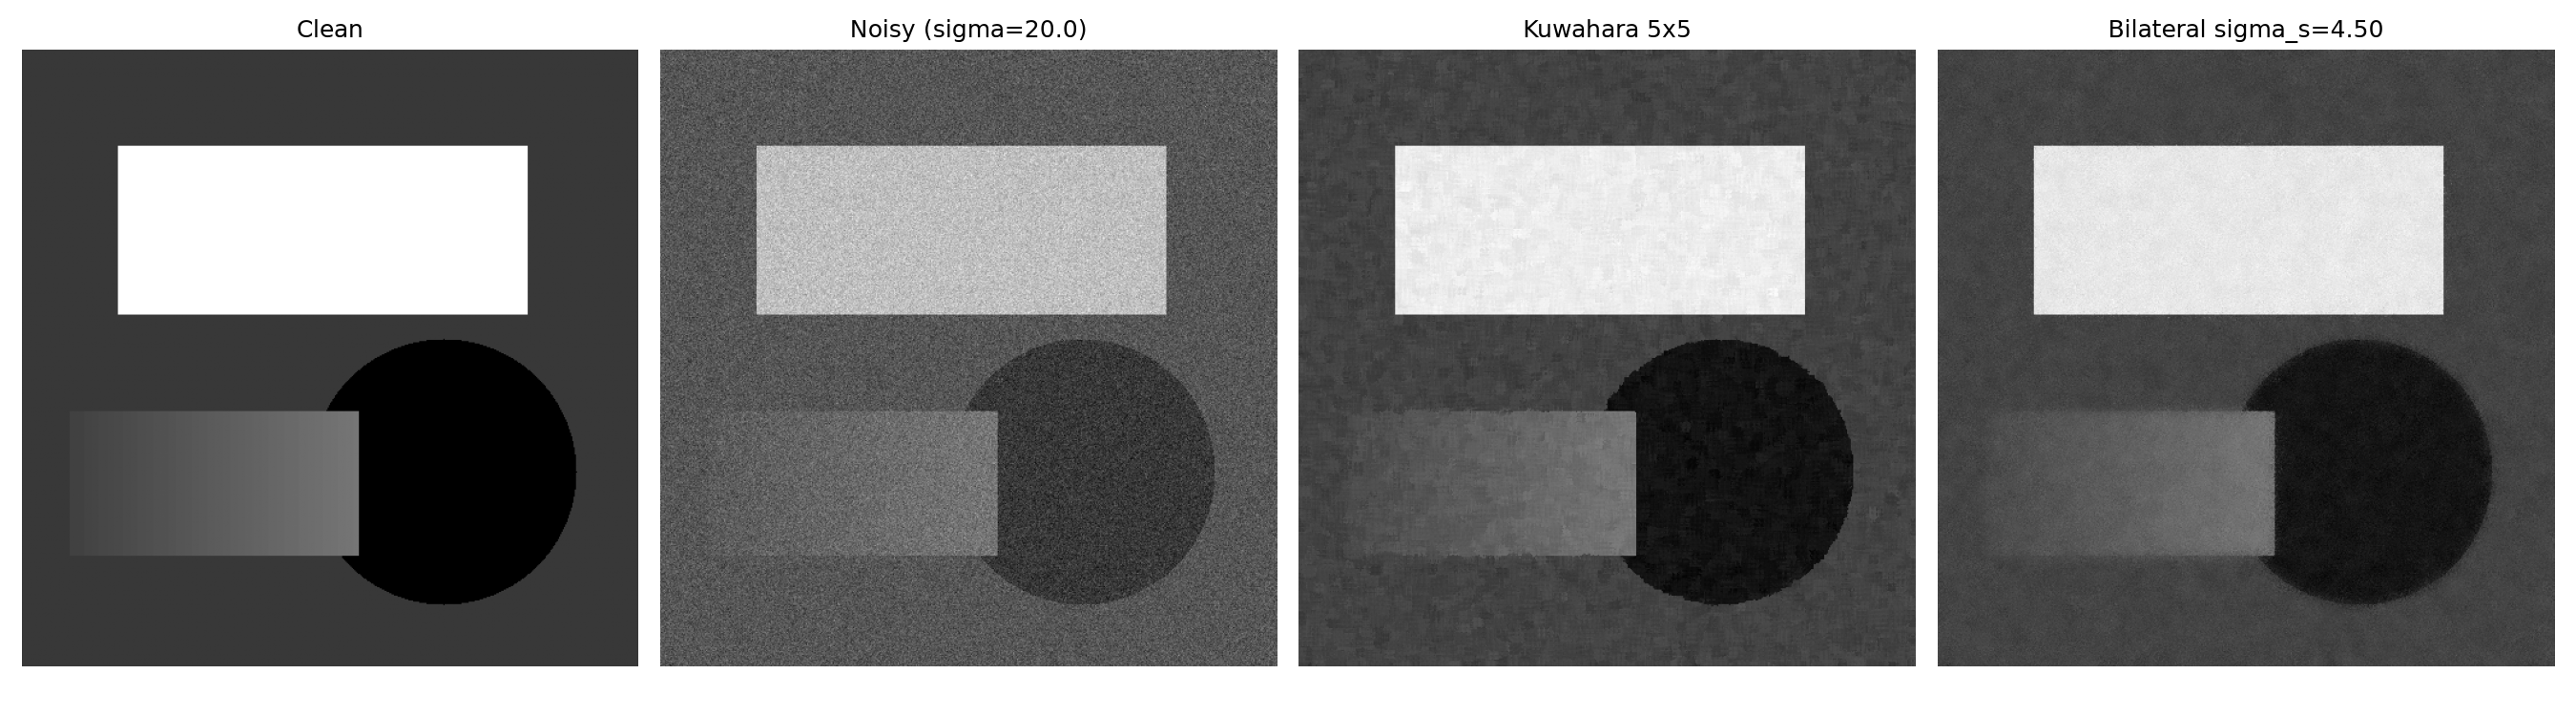
\includegraphics[width=0.8\linewidth]{results/4_1_comparison.png}
  \caption{Full-image comparison: clean ground truth, noisy input ($\sigma=20$), Kuwahara
  output, and bilateral output at matched smoothing strength.}
  \label{fig:41comparison}
\end{figure}

\begin{figure}[H]
  \centering
  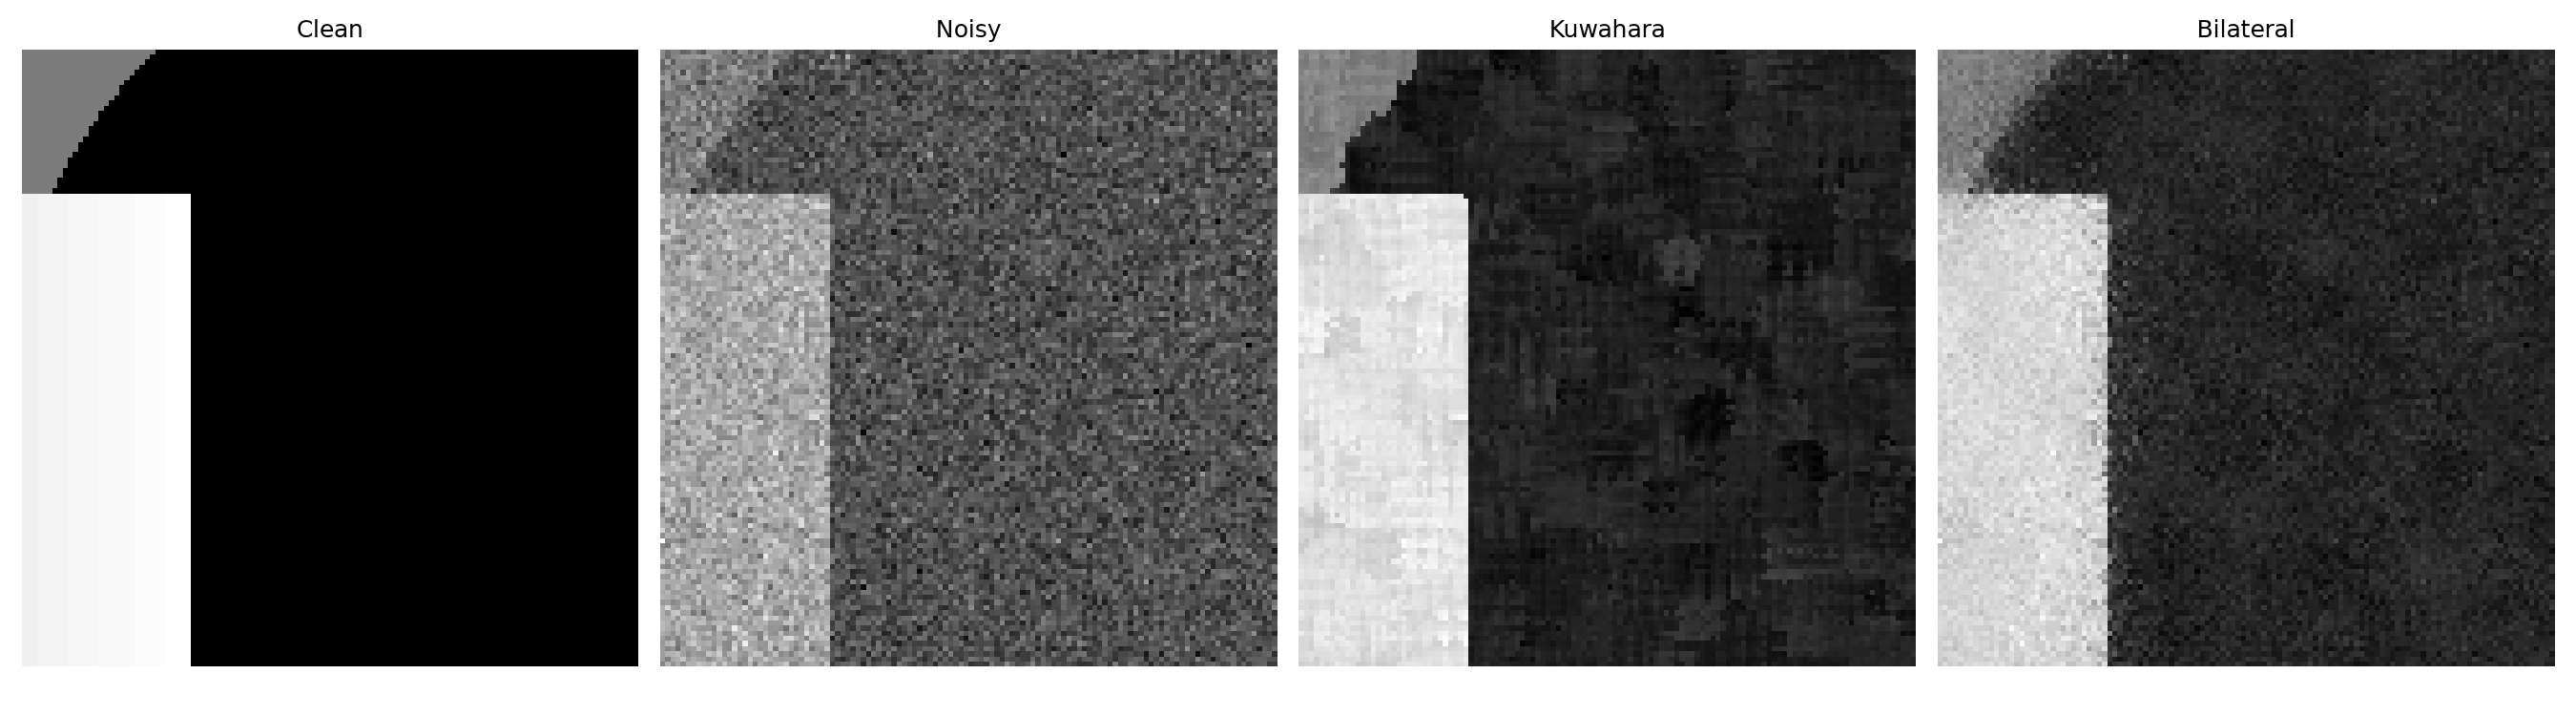
\includegraphics[width=0.8\linewidth]{results/4_1_boundary_zoom.png}
  \caption{Cropped zoom around a circle/rectangle boundary. Kuwahara's edges stay
  visibly crisper -- its sub-window selection actively seeks out the most homogeneous
  side of a boundary, rather than blending across it like an isotropic-footprint average
  -- while bilateral's edge is visibly softer at this matched strength, since bilateral's
  spatial Gaussian still contributes some weight across the boundary even where the range
  kernel down-weights it, whereas Kuwahara's sub-window selection is a hard, all-or-nothing
  choice of an entirely same-side neighbourhood.}
  \label{fig:boundaryzoom}
\end{figure}

Kuwahara edges out bilateral on both PSNR and SSIM here (Table~\ref{tab:psnr_ssim}),
despite matched flat-region denoising strength -- consistent with the visual boundary
comparison of Figure~\ref{fig:boundaryzoom}.

\subsection{Kuwahara de-blocking}

\begin{figure}[H]
  \centering
  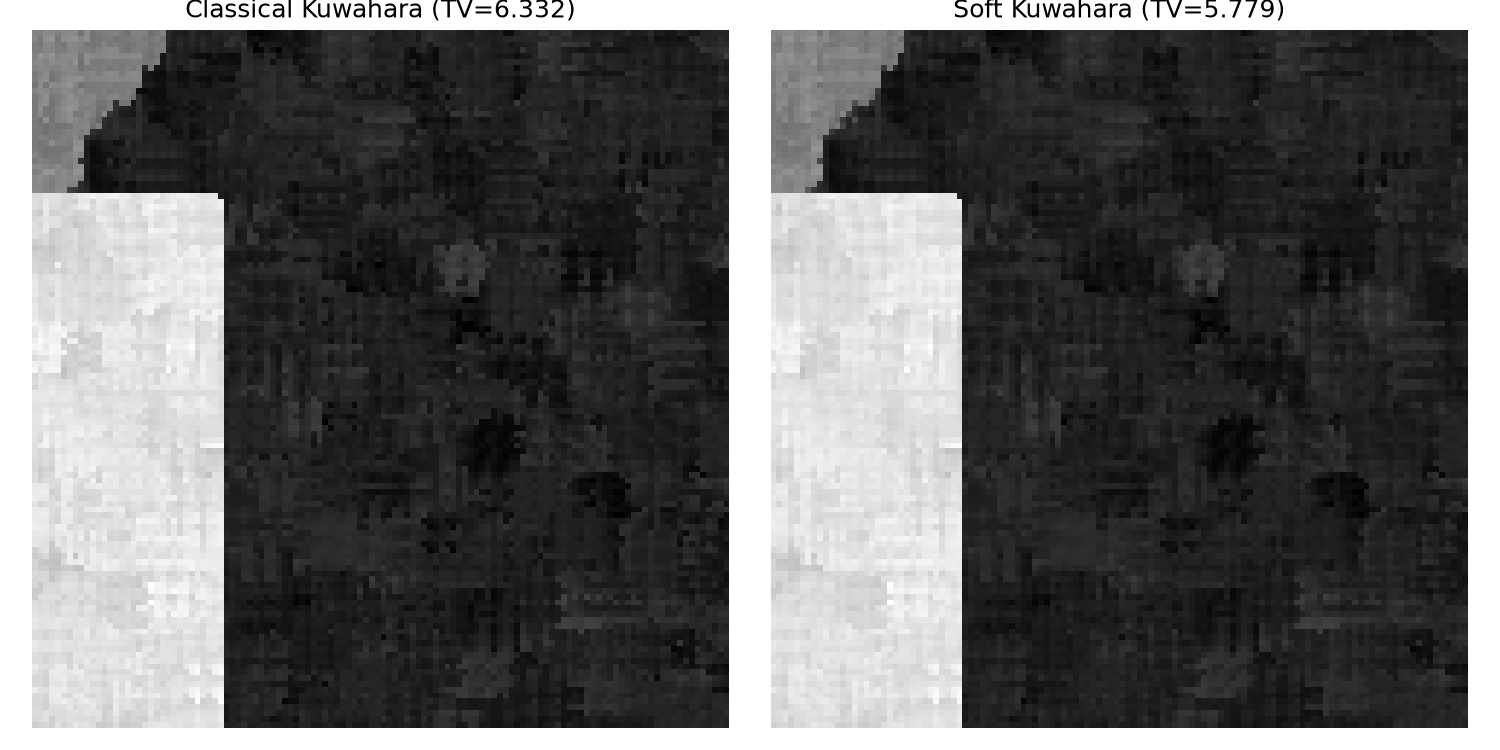
\includegraphics[width=0.8\linewidth]{results/4_2_blockiness_comparison.png}
  \caption{Classical Kuwahara (hard $\arg\min$) vs.\ soft Kuwahara ($T=15$,
  Eq.~\eqref{eq:softkuwahara}) at identical sub-window size. The softmax weighting
  removes the piecewise-constant selection discontinuities responsible for Kuwahara's
  blocky artefacts.}
  \label{fig:blockiness}
\end{figure}

\begin{table}[H]
  \centering
  \caption{Total Variation in a near-edge, still-flat zone, quantifying blockiness
  (exact figures from \texttt{results/4\_2\_result.json}).}
  \label{tab:tv}
  \begin{tabular}{lr}
    \toprule
    Filter & TV in near-edge flat zone \\
    \midrule
    Classical Kuwahara & 6.332 \\
    Soft Kuwahara ($T=15$) & \textbf{5.779} ($-8.7\%$) \\
    \bottomrule
  \end{tabular}
\end{table}

Soft Kuwahara measurably reduces spurious variation right next to true edges, in the
direction predicted by the selection-discontinuity mechanism of Section~2.2.1, though at
$T=15$ the visual difference is subtle; a larger temperature would blend more
aggressively, trading more blockiness reduction for softer edges -- the same
edge-sharpness/artefact trade-off seen throughout this problem.

\begin{table}[H]
  \centering
  \caption{Per-pixel operation counts (analytic, not timed), at the window sizes used in
  this script (Kuwahara sub-window $5\times5\to100$ total taps across 4 sub-windows).
  Two bilateral rows are given: the actual matched filter from Section 4.1
  ($\sigma_s=4.50$, window span $w=29$) and a larger, illustrative $\sigma_s\approx8$
  ($w=49$) to make the $O(w^2)$ scaling trend visible.}
  \label{tab:complexity}
  \begin{tabular}{lrrrrr}
    \toprule
    Algorithm & Taps & Add. & Mult. & Exp. & Comp. \\
    \midrule
    Classical Kuwahara & 100 & 200 & 100 & \textbf{0} & 3 \\
    Soft Kuwahara & 100 & 204 & 104 & \textbf{4} & 0 \\
    Bilateral (matched, $w=29$) & 841 & 2523 & 1682 & \textbf{841} & 0 \\
    Bilateral (illustrative, $w=49$) & 2401 & 7203 & 4802 & \textbf{2401} & 0 \\
    \bottomrule
  \end{tabular}
\end{table}

Bilateral is by far the most computationally expensive per pixel at either window size
tested, because it needs one \texttt{exp()} evaluation for \emph{every single window
tap} ($w^2$ of them -- 841 even at the modest matched $\sigma_s=4.50$, 2401 at the
larger illustrative window) to build the data-dependent range kernel fresh at each
offset, whereas Kuwahara's sub-window statistics (sums and sums-of-squares) only need
cheap additions/multiplications, with the expensive \texttt{exp()} calls limited to a
fixed small constant (0 for hard-argmin classical, 4 for softmax-weighted soft)
regardless of window size -- Kuwahara's exponentiation cost does not scale with its
window at all, while bilateral's scales quadratically with window diameter.

\subsection{Bilateral breakdown under high Noise-to-Contrast Ratio}

\begin{figure}[H]
  \centering
  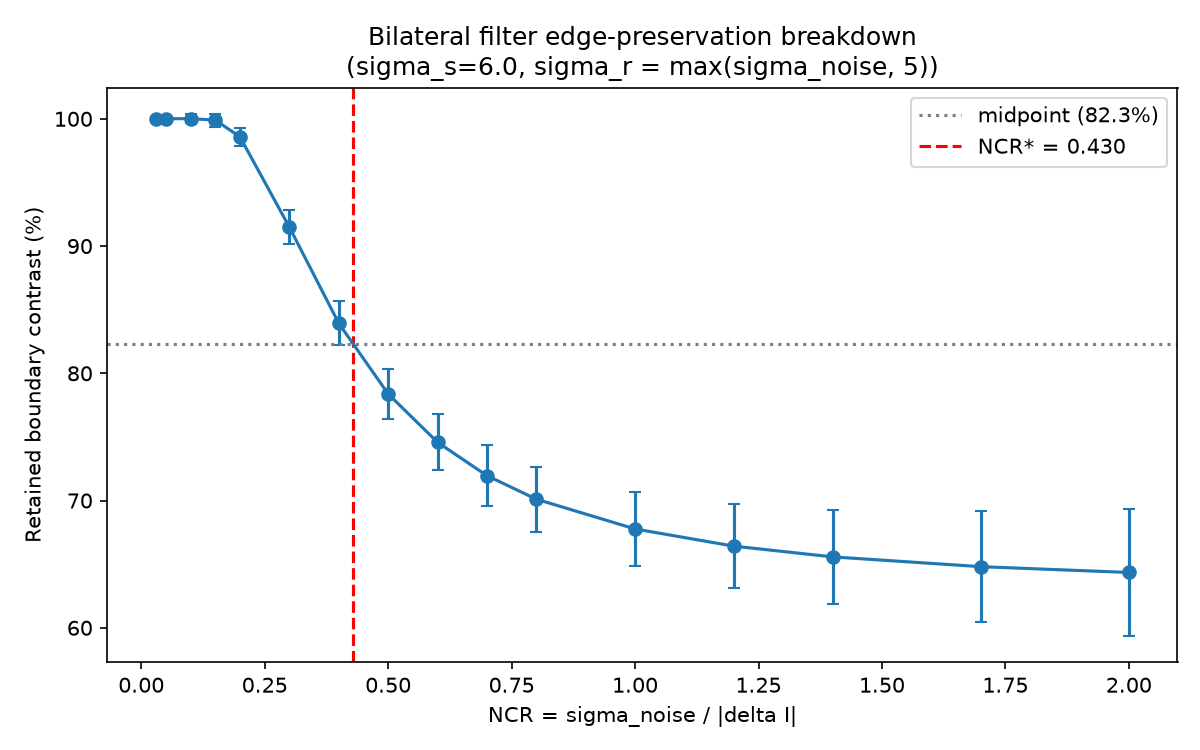
\includegraphics[width=0.8\linewidth]{results/4_3_breakdown_curve.png}
  \caption{Edge-preservation metric (band-averaged retained boundary gradient, \%) vs.\
  NCR, averaged over 6 noise realisations per NCR value. The curve decreases
  monotonically from $\approx100\%$ (NCR $\le 0.15$) to a high-NCR plateau around
  $\approx 65\%$. The critical threshold $\text{NCR}^*=0.430$ (crossing of the midpoint
  between the low and high plateaus, $82.3\%$) is annotated.}
  \label{fig:breakdowncurve}
\end{figure}

\begin{figure}[H]
  \centering
  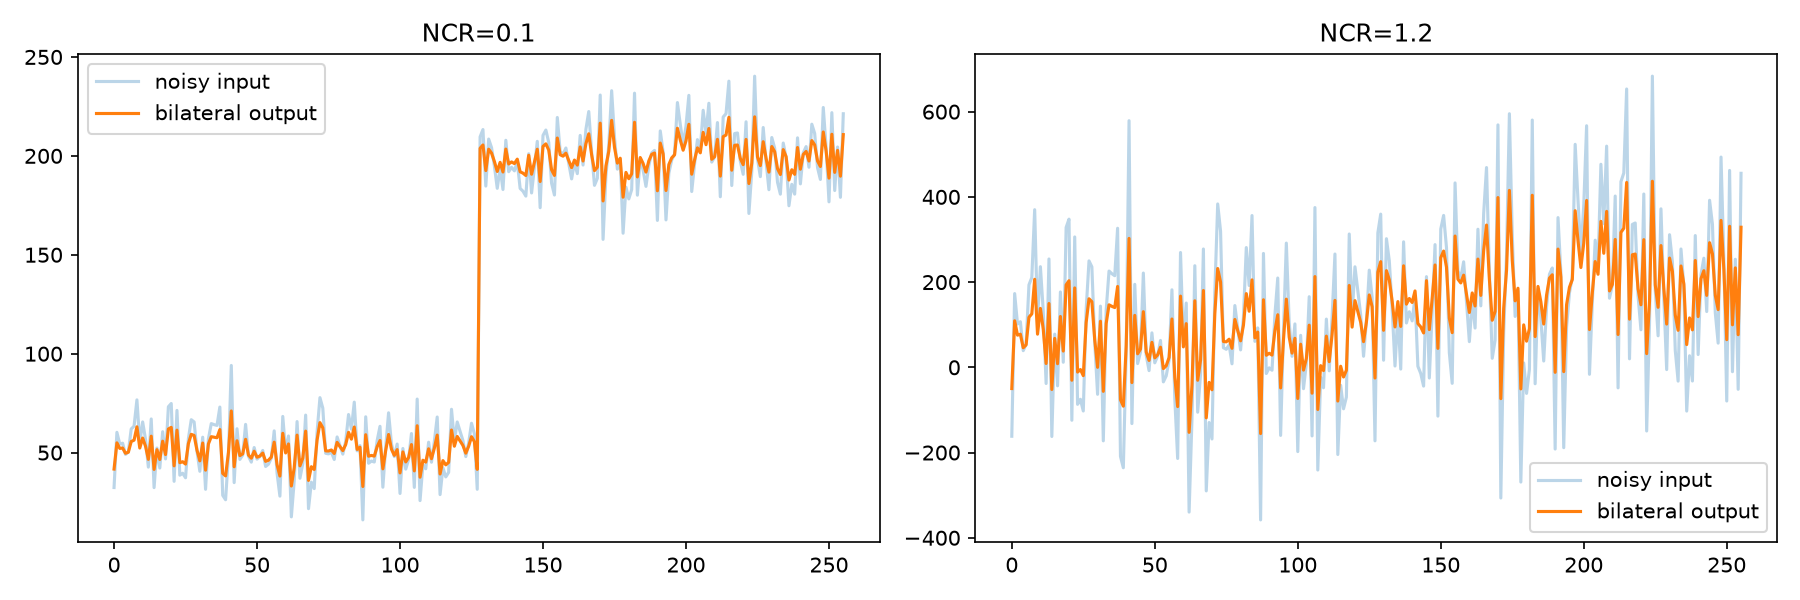
\includegraphics[width=0.8\linewidth]{results/4_3_profiles.png}
  \caption{Example filtered intensity profiles across the step edge at NCR$=0.1$ (edge
  sharply preserved) vs.\ NCR$=1.2$ (visibly smoothed/blended across the boundary).}
  \label{fig:profiles}
\end{figure}

\begin{table}[H]
  \centering
  \caption{Breakdown-curve plateau values and critical ratio (exact figures from
  \texttt{results/4\_3\_result.json}).}
  \label{tab:breakdown}
  \begin{tabular}{lr}
    \toprule
    Quantity & Value \\
    \midrule
    Low plateau (retained \%) & 100.01 \\
    High plateau (retained \%) & 64.58 \\
    Midpoint (retained \%) & 82.29 \\
    $\text{NCR}^*$ & \textbf{0.430} \\
    \bottomrule
  \end{tabular}
\end{table}

The breakdown is sharp and visible between roughly NCR$=0.2$ ($98.6\%$ retained) and
NCR$=0.8$ ($70.1\%$ retained), with $\text{NCR}^*\approx0.43$ falling right in the
middle of that transition -- consistent with the range-kernel analysis of
Section~2.4: at $\text{NCR}^*$, $\sigma_{\text{noise}}$ reaches roughly $43\%$ of the
step height, the point at which the same-side and cross-side typical intensity
differences of Eq.~\eqref{eq:ncrmag} stop being cleanly separable by $w_r$. The curve
plateaus at $\approx65\%$ rather than decaying to $0\%$: once $\sigma_r$ has grown large
enough (recall $\sigma_r=\sigma_{\text{noise}}$ at high NCR under the adaptive rule) to
no longer discriminate same- vs.\ cross-side pairs at all, the filter degenerates toward
a pure spatial Gaussian average with no range restriction; measured 4 pixels off-centre
from the boundary, even a pure spatial blur with $\sigma_s=6$ retains a non-zero
fraction of the step contrast at that offset, rather than averaging it away completely,
hence the plateau sits well above, not at, $0\%$.

\section{Conclusion}

This problem implemented and rigorously compared two structurally different
edge-preserving smoothing filters. At a quantitatively matched smoothing strength
(equal variance-reduction factor on a flat noisy patch), classical Kuwahara outperformed
the bilateral filter on both PSNR ($35.40$ vs.\ $34.57$ dB) and SSIM ($0.850$ vs.\
$0.788$), and preserved visibly crisper edges, because its hard sub-window selection
makes an all-or-nothing choice of an entirely same-side neighbourhood rather than
blending some cross-edge weight in as bilateral's isotropic spatial kernel does. That
same hard-selection mechanism, however, is responsible for Kuwahara's characteristic
blocky artefacts, traced here to discontinuous flips in which sub-window ``wins'' as the
window slides -- distinct from both blur and ringing -- and measurably (though modestly,
$-8.7\%$ TV) mitigated by a softmax (soft-Kuwahara) reformulation. A per-pixel operation
count further showed that bilateral filtering, despite its elegant formulation, is by
far the most computationally expensive of the three algorithms, since it requires one
exponential evaluation per window tap rather than a small, window-size-independent
constant. Finally, a controlled synthetic experiment located and mathematically
explained a sharp breakdown in bilateral filtering's edge-preservation ability at
$\text{NCR}^*\approx0.43$: once noise standard deviation approaches a sizeable fraction
of the step height, the range kernel can no longer statistically distinguish same-side
noise from cross-side signal, and the filter degrades toward an edge-blind spatial blur.

\end{document}
